\documentclass[journal]{IEEEtran}
\IEEEoverridecommandlockouts
\usepackage{graphics}
\usepackage{rotating}
\usepackage{epsfig}
\usepackage{amsmath}
\usepackage{amssymb}
\usepackage{eqnarray}
\usepackage[spanish, es-tabla]{babel}
\usepackage{cite}
\usepackage{hyperref}
\usepackage{float}
\usepackage{csvsimple}
\usepackage[justification=centering]{caption}
\usepackage{atbegshi} % erase first blank page
\AtBeginDocument{\AtBeginShipoutNext{\AtBeginShipoutDiscard}}
\spanishdecimal{.}

\title{\LARGE \bf Análisis de Riesgo de una Compañía Aseguradora}

%%%%%%%%%%%%%%%%%%%%%% AUTHORS %%%%%%%%%%%%%%%%%%%%%%%%%%%%%%%%%%%%%%%%5
\author{Juan Pablo Echeagaray González, Verónica Victoria García De la Fuente, \\ Emily Rebeca Méndez Cruz, Eugenio Santiesteban Zolezzi, \\ Daniel De Zamacona Madero \\
Optimización Estocástica \\
MA2004B.101 \\
Dr. Fernando Elizalde Ramírez \\
Dr. Jaime Eduardo Martínez Sánchez}

\begin{document}

    \thanks{Juan Pablo Echeagaray González, Verónica Victoria García De la Fuente, Emily Rebeca Méndez Cruz, Eugenio Santiesteban Zolezzi, Daniel De Zamacona Madero pertencen al Tec de Monterrey Monterrey, N.L. C.P. 64849, Mexico {\tt\small}}
    
    \maketitle
    
    \thispagestyle{empty}
    \pagestyle{empty}
    %%%%%%%%%%%%%%%%%%%%%%%%%%%%%%%%%%%%%%%%%%%%%%%%%%%%%%%%%%%%%%%%%%%%%%%%%%%%%
    \begin{abstract}
       Una empresa aseguradora ha solicitado que alumnos del Tecnológico de Monterrey estimen la probabilidad de ruina de su empresa a horizontes de tiempo finito e infinito. Con la base de datos recibida se realizaron análisis estadísticos para aplicar el modelo de \emph{Cramér-Lundberg} para la estimación de la probabilidad de ruina. Se calculó dicha probabilidad mediante simulación Monte Carlo y por la fórmula de \emph{Pollaczek-Khinchine}.
    \end{abstract}
    
    \begin{IEEEkeywords} 
        Probabilidad de Ruina, Pollaczek-Khinchine, Monte Carlo
    \end{IEEEkeywords}
    %%%%%%%%%%%%%%%%%%%%%%%%%%%%%%%%%%%%%%%%%%%%%%%%%%%%%%%%%%%%%%%%%%%%%%%%%%%%%%%%
    \section{Introducción} \label{sec:introduction}
    
        El riesgo se define como la posibilidad de perder algo o de tener un resultado no deseado, negativo o peligroso. Este se divide en dos componentes: la probabilidad de que un resultado negativo suceda, y el tamaño de dicho resultado; por lo que tenemos que mientras mayor sea la probabilidad y la pérdida potencial, mayor será el riesgo que se presente \cite{risk-definition}.
        
        El análisis de riesgo financiero evalúa dicha probabilidad y mediante su estimación, se combina la ocurrencia del riesgo y las posibles perdidas. Con esto buscamos investigar la probabilidad de ruina de una empresa de seguros realizando un modelo que simule distintas réplicas de la problemática.

        Este escrito se organiza de la siguiente manera: en las secciones \ref{sec:problem-description} y \ref{sec:research-questions} se presenta la problemática a resolver y se plantean las preguntas de investigación que dirigirán nuestro análisis. En la sección \ref{sec:theoretical-framework} se presentan algunos conceptos teóricos de Teoría de Riesgo necesarios para comprender la relevancia de nuestro proyecto.

        En las secciones \ref{sec:method} y \ref{sec:proposed-method} se presenta la metodología seguida así como los análisis estadísticos necesarios para el cálculo de la probabilidad de ruina; después presentamos los resultados de nuestras estimaciones en la sección \ref{sec:results} para después discutir las áreas de oportunidad encontradas en la sección \ref{sec:discussion}. Finalmente presentamos las conclusiones de nuestro estudio en la sección \ref{sec:conclusions}.

        En las secciones \ref{sec:resources} y \ref{sec:source-code} se presentan datos técnicos del equipo utilizado y se proporciona una liga al código fuente implementado.
        
    \section{Descripción de la problemática} \label{sec:problem-description}
    
        El reto se enfoca en el análisis del riesgo financiero concentrándose concretamente en las pérdidas económicas que surgen del pago que debe de hacer la compañía ante el caso de un siniestro, si el monto total de pagos exceden el capital que tiene disponible la compañía se producirá su ruina y provocará que salga del mercado. 
    
        \subsection{Modelo clásico de Cramér-Lundberg}\label{cap:CL}
        
            Para definir este modelo se toman en cuenta diversos aspectos como el capital inicial de la compañía, el monto recibido por unidad de tiempo, tamaño y número de reclamos en determinados momentos; todas estas variables proyectadas contra reclamaciones en tiempos aleatorios $W_1, W_2, \ldots$ de acorde a un proceso de Poisson homogéneo $\left\{N(t): t > 0\right\}$ con una intensidad $\lambda > 0$. Este supuesto implica que los tiempos entre las llegadas de los eventos son variables aleatorias independientes e idénticamente distribuidas con distribución común exponencial \cite{ekaterina}. Aunado a esto se hipotetiza que los tamaños de estas reclamaciones siguen una distribución común $F$ de cola ligera, con las siguientes propiedades:
            \begin{gather*}
                F(0) = 0 \\
                E(Z_k) = \mu >0
            \end{gather*}

            La compañía recibe de sus asegurados una prima constante mayor a cero por unidad de tiempo, por lo que al denotar X(t) como el capital de la compañía en tiempo $t$, se tiene que
            \begin{equation}\label{eqn:classical-cramer}
                X(t) = u + ct -\sum_{k=1}^{N(t)}Z_k
            \end{equation}

            De forma intuitiva podemos decir que $\sum_{k=1}^{0}$ es igual a cero, esto hace alusión a que si no hubo ningún siniestro, no podemos suponer que la empresa tendrá que realizar un pago; y que el índice superior de la sumatoria, $N(t)$ es el número de reclamos en el intervalo $(0,t]$. Esta definición de $X(t)$ resulta como el modelo clásico de riesgo, el modelo de \emph{Cramér-Lundberg}.

            Para efectos prácticos de modelado y simulación, hemos optado por modificar la nomenclatura básica del modelo de \emph{Cramér-Lundberg} a la siguiente fórmula iterativa:
            \begin{equation}\label{eqn:iterative-cramer}
                \begin{aligned}
                    X(0) &= U_0 \\
                    X(t+1) &= X(t) + c -\sum_{k=1}^{N(t)}Z_k
                \end{aligned}
            \end{equation}

            Un desglose algebraico de la ecuación \ref{eqn:iterative-cramer} es suficiente para ver que es equivalente a la ecuación \ref{eqn:classical-cramer} del modelo original.
            
    \section{Preguntas de investigación} \label{sec:research-questions}

        Mediante el análisis de la base de datos que nos ha proporcionado el Socio Formador, nos planteamos 2 preguntas con el fin de guiar nuestro estudio:
    
        \begin{enumerate}
            \item ¿Cuál es la probabilidad de que la compañía aseguradora caiga en ruina en un tiempo finito $T$?
            \item ¿Cuál es la probabilidad de que la compañía aseguradora caiga en ruina para un horizonte de tiempo infinito?
        \end{enumerate}
        
        Para ambas preguntas se adjuntan posibles alteraciones al modelo para mejorar la predicción y control de los episodios donde la compañía tenga que solventar gastos de siniestros y ampliar la predicción en un plazo de tiempo continuo con duración infinita.
        
        Con esto introducimos las cargas de seguridad para las primas, las cuales se vincularían con las primas recolectadas y un factor de carga acompañado por la seriedad de los siniestros, mediante el factor de carga podemos indicar si las primas incitan un mayor riesgo de ruina o si la clientela preferiría buscar otras alternativa. Para la el estado continuo en tiempo infinito tiene como objetivo proporcionar un límite superior para la probabilidad de ruina, usando la desigualdad de Lundberg ajustamos mediante el coeficiente $R$ una medida inversa de riesgo que mientras mayor sea menor es el límite superior. Para el proceso compuesto de Poisson con parámetro $\lambda$, obtenemos una $R$ raíz única positiva de la ecuación:
        
        \begin{equation}
            \lambda + cr = \lambda M_x(r)
        \end{equation} 
        
        Con $\lambda$ siendo el parámetro de poisson, $c$ la prima de tasa de unidad de tiempo, y $M_x(r)$ es la función generadora de momentos para el indicador de reclamos en cierto punto, con esto es posible derivar el límite superior e inferior para $R$ y así generalizar el modelo para incluir el impacto del reaseguro en caso de ruina.

    \section{Marco teórico} \label{sec:theoretical-framework}

        Cada que se tome una decisión se debe valorar la relación costos-beneficios, de lo contrario no estaríamos evaluando los riesgos que se corren al tomar dicha decisión y las ventajas o desventajas que esta nos traería \cite{risk-definition}.
            
        Existen riesgos cuando los posibles escenarios con sus resultados son conocidos y existen antecedentes para la estimación de su distribución de frecuencia \cite{Bazzani}. El riesgo financiero, también llamado riesgo de crédito o de insolvencia, es considerado como el riesgo de pérdidas en las posiciones dentro y fuera del balance proveniente de movimientos adversos en los precios de mercado. Este hace referencia a la incertidumbre asociada al rendimiento de la inversión debido a la posibilidad de que la empresa no pueda afrontar sus obligaciones financieras, como lo son el pago de los intereses y la amortización de las deudas. Las obligaciones financieras fijas en las que incurren es el único factor por la que ocurre el riesgo financiero \cite{Bazzani}.
        
        En cuanto a la compañía aseguradora, el modelo de negocios se representa con la relación de ingresos por primas devengadas e inversiones y de egresos por siniestros y gastos de emisión. Tenemos que la aseguradora aumenta sus ingresos mediante dos alternativas \cite{aseguradora}:
        \begin{itemize}
            \item Aumento de la prima devengada, esta se logra a través del aumento de pólizas  subscritas o mejora de cartera.
            \item Manejo óptimo del portafolio de clientes, esto se genera mediante decisiones de inversión que generen el mayor retorno posible.
        \end{itemize}
        
        Respecto a la disminución de los egresos de la aseguradora, esta se produce por medio de dos alternativas \cite{aseguradora}:
        \begin{itemize}
            \item Optimización de los cálculos de reservas para cubrir los siniestros.
            \item Disminución de los gastos de emisión, reduciendo gastos como comisiones y exámenes médicos, así también las pólizas que se cancelan.
        \end{itemize}
        
        Durante el proyecto se hará uso del modelo de Cramér-Lundberg para la definición del modelo clásico de riesgo, como lo hemos descrito anteriormente \ref{cap:CL}.
        
    \section{Metodología} \label{sec:method}

        Se realizará una limpieza de la base de datos proporcionada por el Socio Formador; se comprobará la independencia de los montos de los siniestros y la cantidad de siniestros por día mediante una prueba de correlación, después se determinarán las distribuciones que modelan la frecuencia de ocurrencia de los siniestros así como los montos pagados por la aseguradora por cada uno de ellos mediante pruebas de bondad de ajuste; se procederá después a estimar los parámetros de dichas distribuciones con las pruebas de hipótesis correspondientes, se brindarán también intervalos de confianza para cada parámetro estimado.

        Con los parámetros estimados con anterioridad se determinará primero una expresión para la prima $c$ que garantice una probabilidad de ruina diferente a 1. Con estos parámetros se realizará una simulación de la probabilidad de ruina de la aseguradora a un horizonte finito $T$. Finalmente se calculará la probabilidad de ruina a un horizonte de tiempo infinito mediante la fórmula de \emph{Pollaczeck-Kinchine} \cite{josafat-santana-2020}.
    
    \section{Propuesta metodológica} \label{sec:proposed-method}

        Para la solución de esta problemática hemos usado el lenguaje de programación \texttt{Python} en su versión 3.10.4; para los procesos de lectura, limpieza, exploración y agregación de datos hemos usado la librería \texttt{pandas} \cite{pandas} en conjunto con \texttt{matplotlib} \cite{matplotlib} y \texttt{seaborn} \cite{seaborn}, para las pruebas de hipótesis correspondientes así como para la generación de números aleatorios de acuerdo a las distribuciones encontradas se utilizó el módulo \texttt{stats} de la librería \texttt{scipy} \cite{scipy} y la librería \texttt{statsmodels} \cite{seabold2010statsmodels}. Una liga al código fuente desarrollado se encuentra en el apéndice.

        \subsection{Limpieza de la base de datos}

            Se recibió una base de datos de una empresa aseguradora de coches en formato \texttt{csv}, en esta se incluyen los diferentes siniestros ocurridos en determinado tiempo. Se tienen la fecha del mismo, el tipo de auto, el modelo, el monto del siniestro, si se aplica la cobertura, la cantidad del deducible, si el cliente aplicó el seguro y si el siniestro representó una pérdida total.
        
            Se aplicó un proceso de limpieza de datos en la que se removieron todos los siniestros en los que no se aplicó el seguro con el fin de tener solamente los datos que sí generaron una pérdida económica para la empresa aseguradora.

        \subsection{Validación de los supuestos del modelo}

            Para este caso de estudio se necesitan demostrar 3 supuestos; el que los montos de los reclamos sean independientes de la frecuencia de los siniestros, que la frecuencia de siniestros pueda ser modelada como un proceso de Poisson Homogéneo y que la distribución del monto de los reclamos $F$ sea de cola ligera, estos supuestos vienen del artículo de la Dra. Ekaterina \emph{Probabilidad de ruina en el modelo clásico de Cramér-Lundberg} publicado en el 2011 \cite{ekaterina}.

            En cada prueba de hipótesis y cálculo de intervalos de confianza en el presente escrito se utilizará un nivel de significancia $\alpha$ de $0.05$.

            \subsubsection{Prueba de independencia}
            
                El primer paso en nuestro estudio será verificar que exista independencia entre el monto de los reclamos y el número de reclamos por día; la modelación que seguimos originalmente propuesta por la Dra. Ekaterina en \cite{ekaterina} asume que existe independencia entre estas 2 variables, en caso contrario, no podremos utilizar el modelo de \emph{Cramér-Lundberg}. Como un primer heurístico, podemos visualizar estas 2 variables en el diagrama de dispersión que presentamos en la figura \ref{img:scatter-independence}.
                \begin{figure}[!htbp]
                    \centering
                    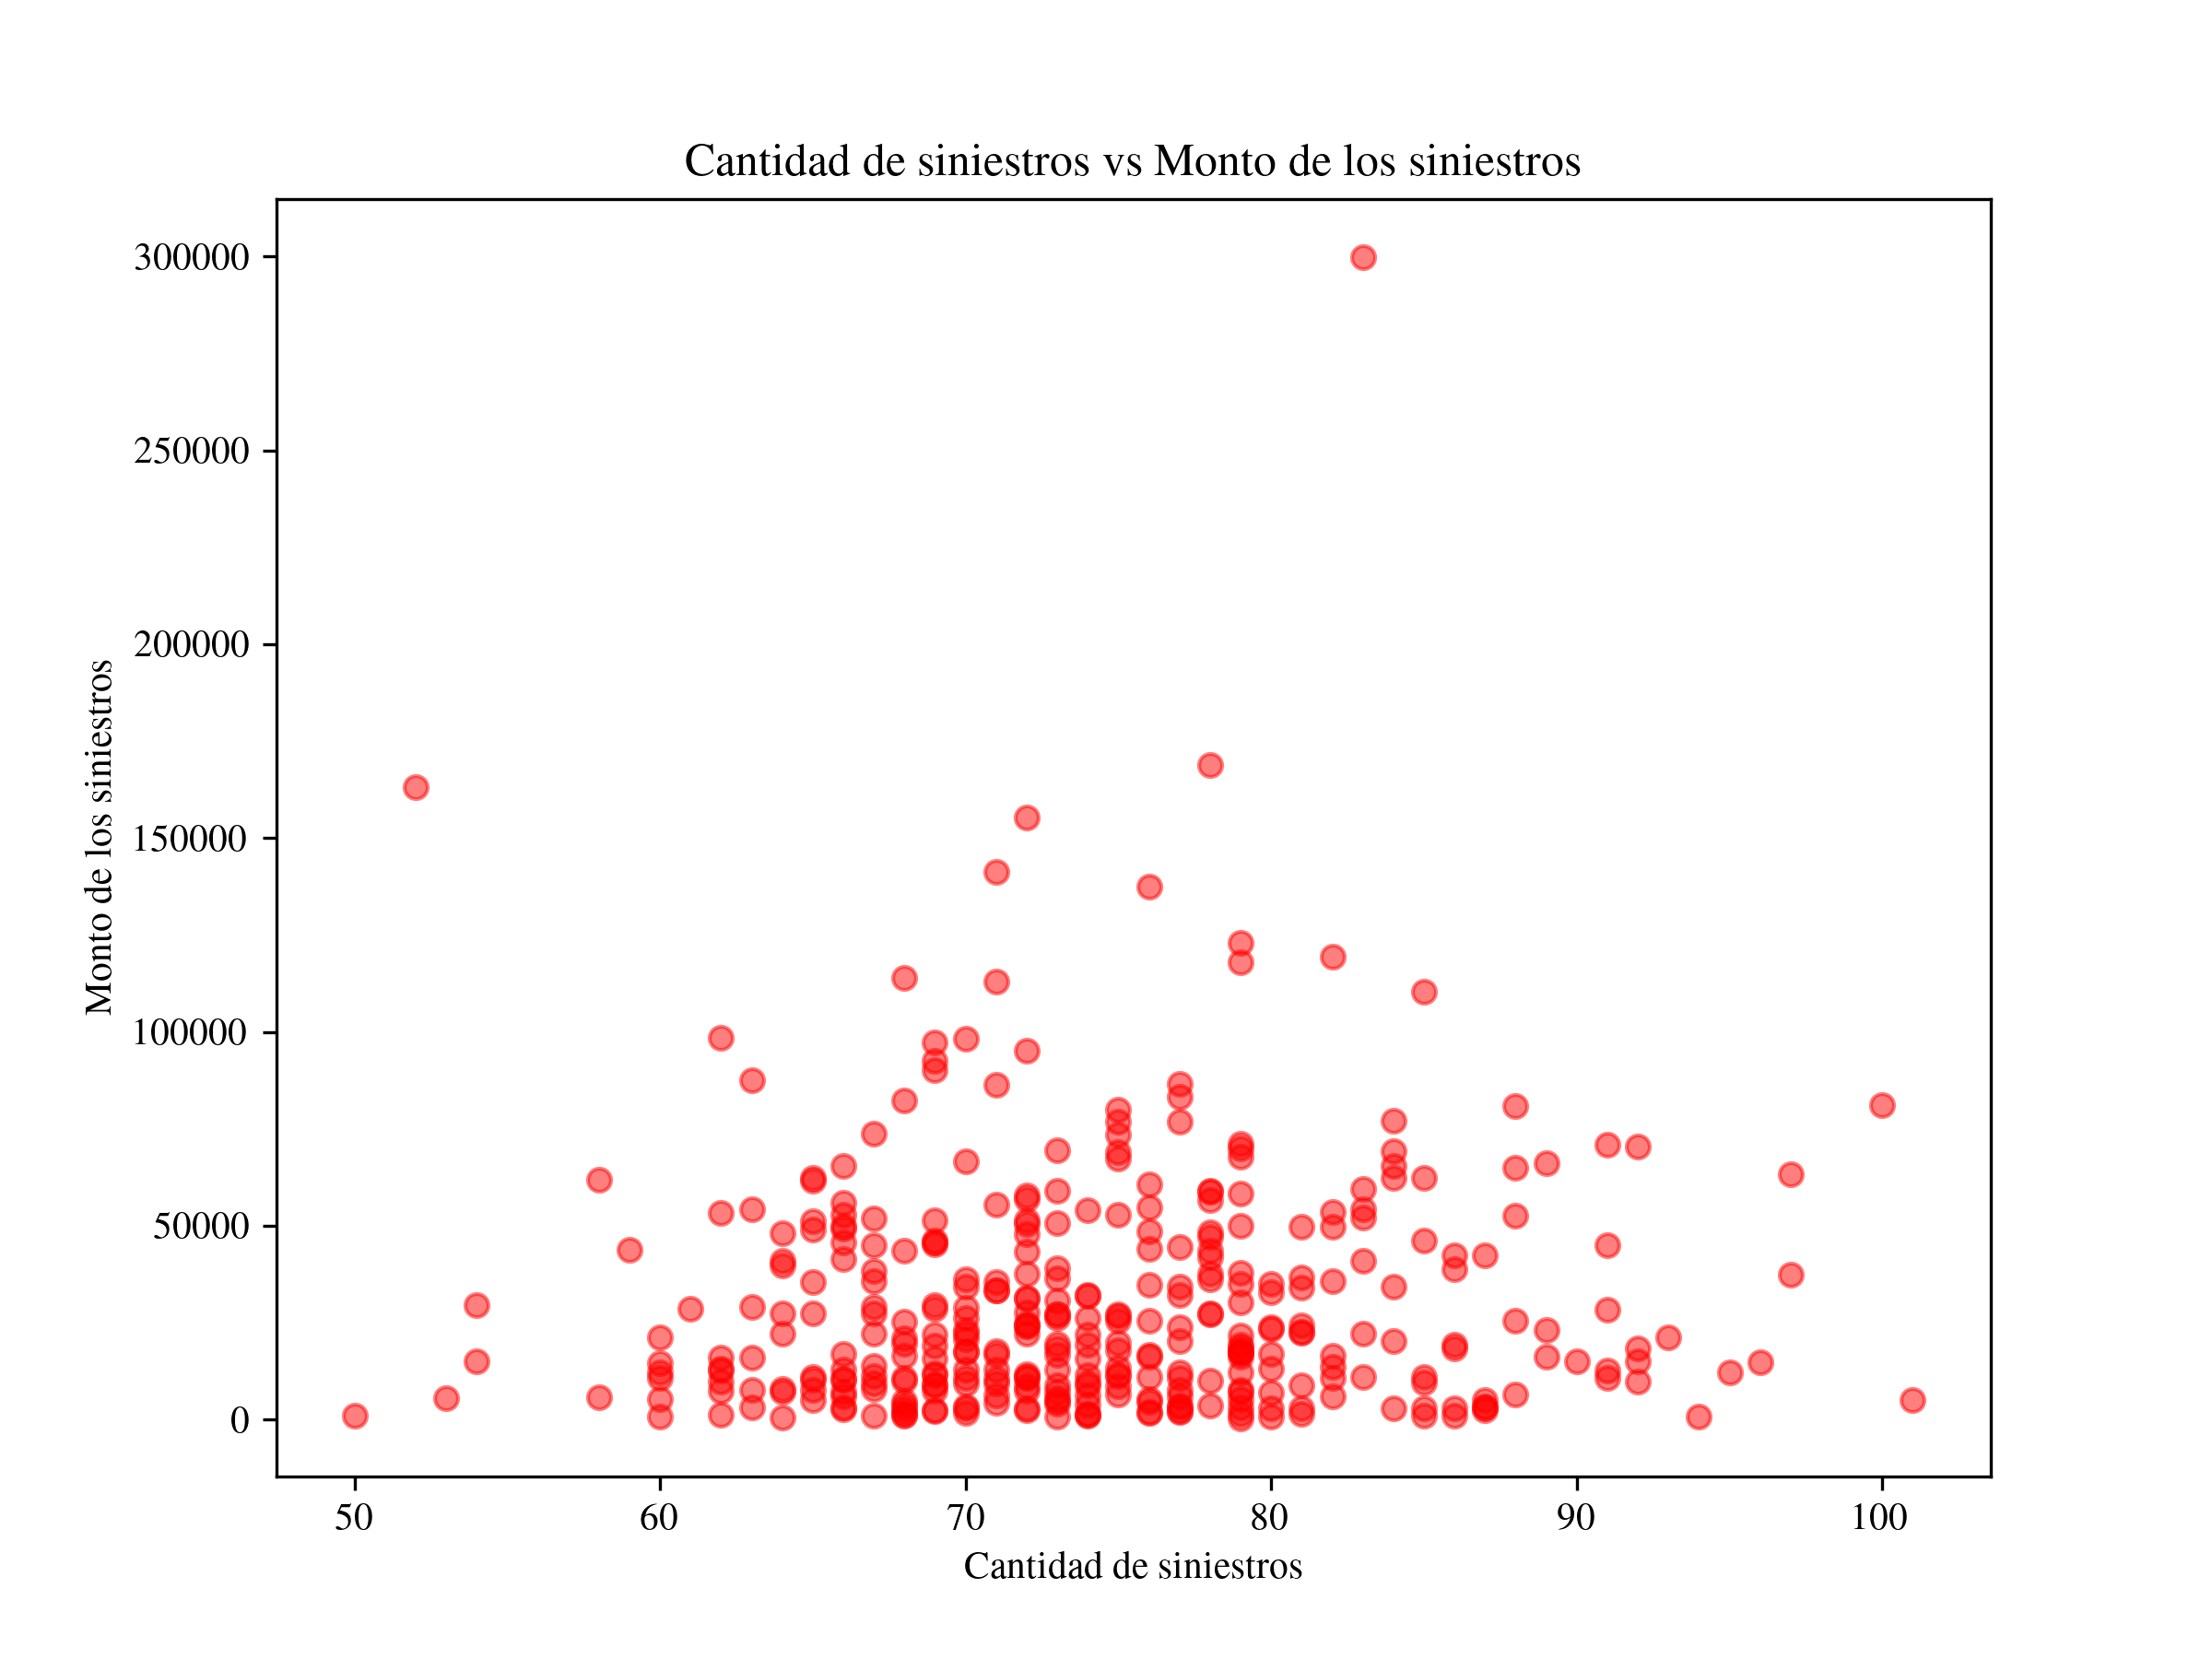
\includegraphics[scale=0.45]{img/independent.png}
                    \caption{Diagrama de dispersión del monto de los siniestros contra la cantidad de reclamos por día}
                    \label{img:scatter-independence}
                \end{figure}

                De forma intuitiva, podemos ver que no existe una relación aparente con los datos; se formalizará ahora este supuesto mediante una prueba de hipótesis para el coeficiente de correlación $\rho$ de Spearman ya que puede medir dependencias más allá de una lineal, con un nivel de significancia $\alpha = 0.05$
                \begin{gather*}
                    H_0: \rho = 0 \\
                    H_1: \rho \neq 0
                \end{gather*}

                Encontramos que el coeficiente de correlación para estas 2 variables es $\rho = 0.06501$. El \textit{p-value} obtenido de esta prueba fue $0.215$, por lo tanto, no podemos rechazar la hipótesis nula, supondremos que existe independencia entre estas 2 variables.
            
            \subsubsection{Distribución de la frecuencia de los reclamos}
            
                Realizaremos una prueba de bondad de ajuste \textit{chi-square} para las cantidad de siniestros, $N(t)$ que hay un dado periodo. En la figura \ref{img:claims_per_day} presentamos el comportamiento de este proceso de conteo en la muestra recibida. 
            
                \begin{figure}[!htbp]
                    \centering
                    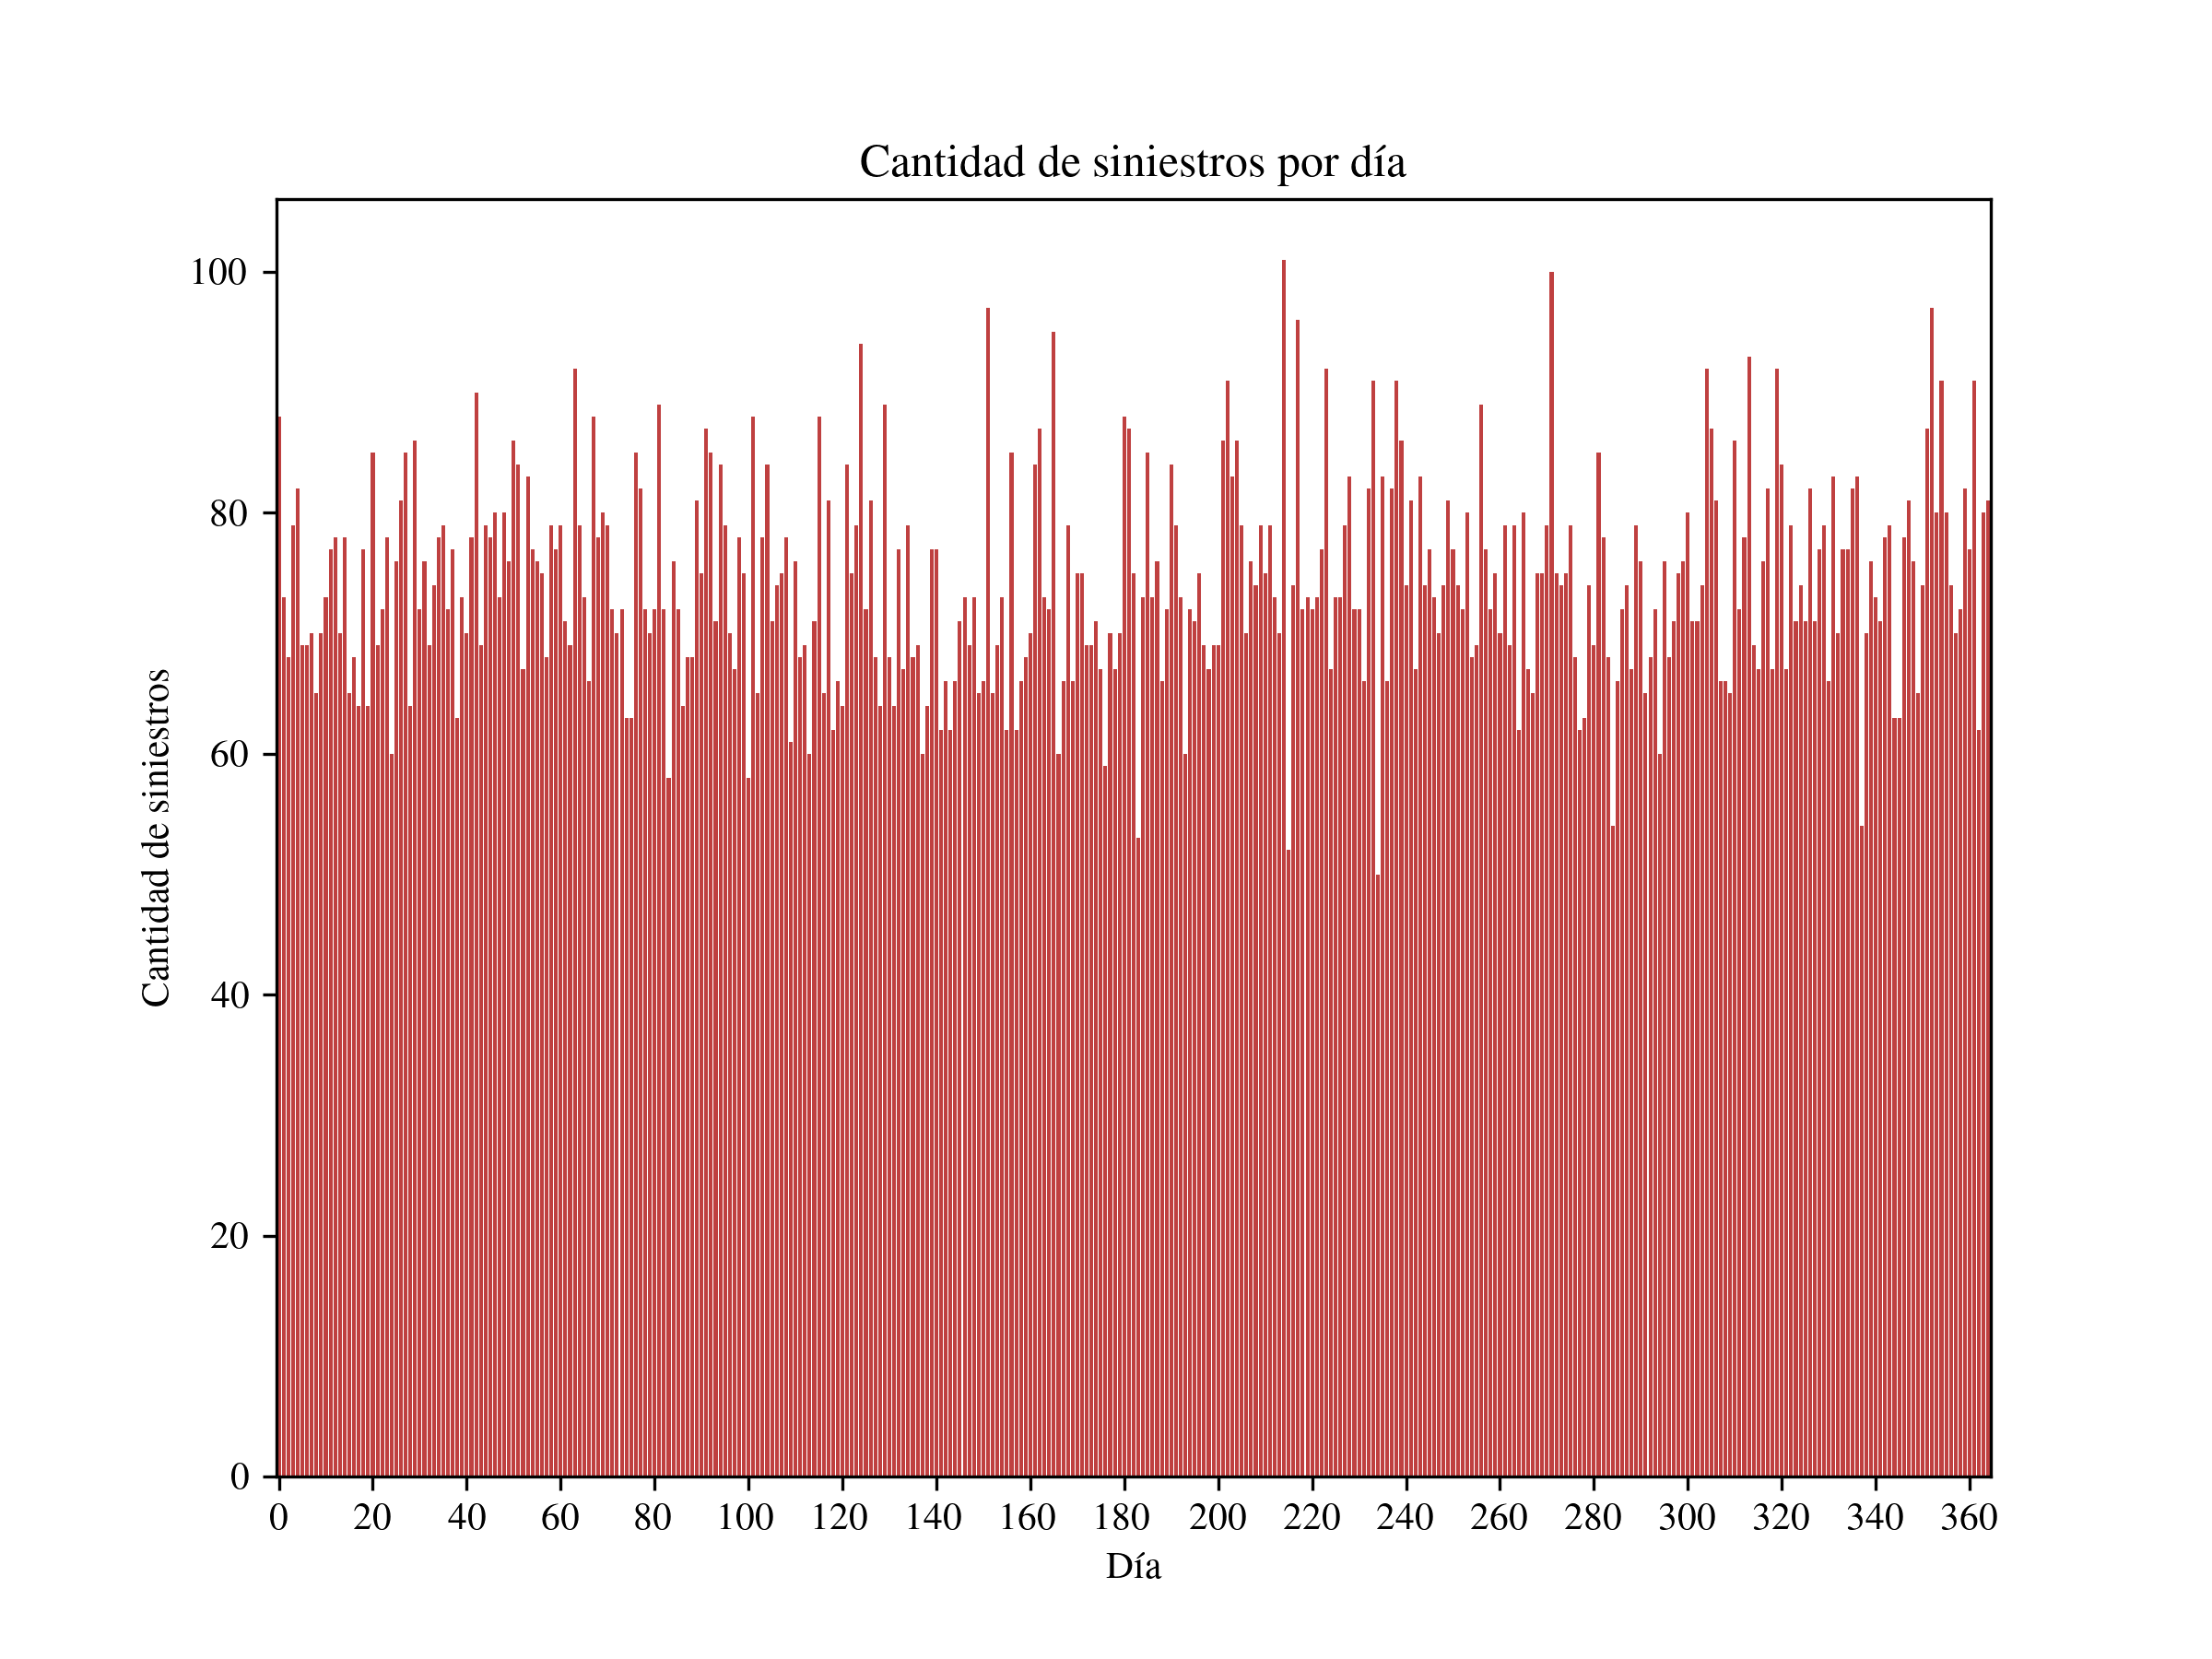
\includegraphics[scale=0.45]{img/claims_per_day.png}
                    \caption{Distribución de la frecuencia de reclamos por día}
                    \label{img:claims_per_day}
                \end{figure}

                Como esperamos modelar esta cantidad como proveniente de un proceso de Poisson homogéneo, se realiza una prueba de bondad de ajuste para la distribución de Poisson; realizamos esta prueba con un nivel de significancia $\alpha = 0.05$. Las hipótesis nula y la hipótesis alternativa que planteamos son entonces:
                \begin{gather*}
                    H_0: N(t) \sim \text{Poisson}(\lambda t) \\
                    H_1 : N(t) \not \sim \text{Poisson}(\lambda t)
                \end{gather*}

                El estadístico de prueba obtenido fue de $16.1425$ con un \textit{p-value} de $0.373$, el cual es mayor nuestro nivel de significancia, por lo que no se puede rechazar la hipótesis nula, podemos continuar nuestro estudio suponiendo que la cantidad de reclamos en cada día puede ser modelado como un proceso de Poisson homogéneo.

            \subsubsection{Distribución del monto de los reclamos}

                Para el caso de la distribución del monto de los reclamos haremos la prueba de \textit{Anderson-Darling}\cite{evans2008distribution} y aplicaremos la prueba de \emph{Lilliefors} \cite{lilliefors1969kolmogorov} para la distribución exponencial. Hemos decidido realizar 2 pruebas de bondad de ajuste dado que uno de los supuestos más fuertes de nuestro modelado es que la distribución del monto de los reclamos es de cola ligera; el que la cola sea pesada dificultará enormemente la determinación de la fórmula analítica de la probabilidad de ruina a un horizonte infinito. Se muestra una visualización de la distribución de los montos en la figura \ref{img:amount-dist}.
                \begin{figure}[!htbp]
                    \centering
                    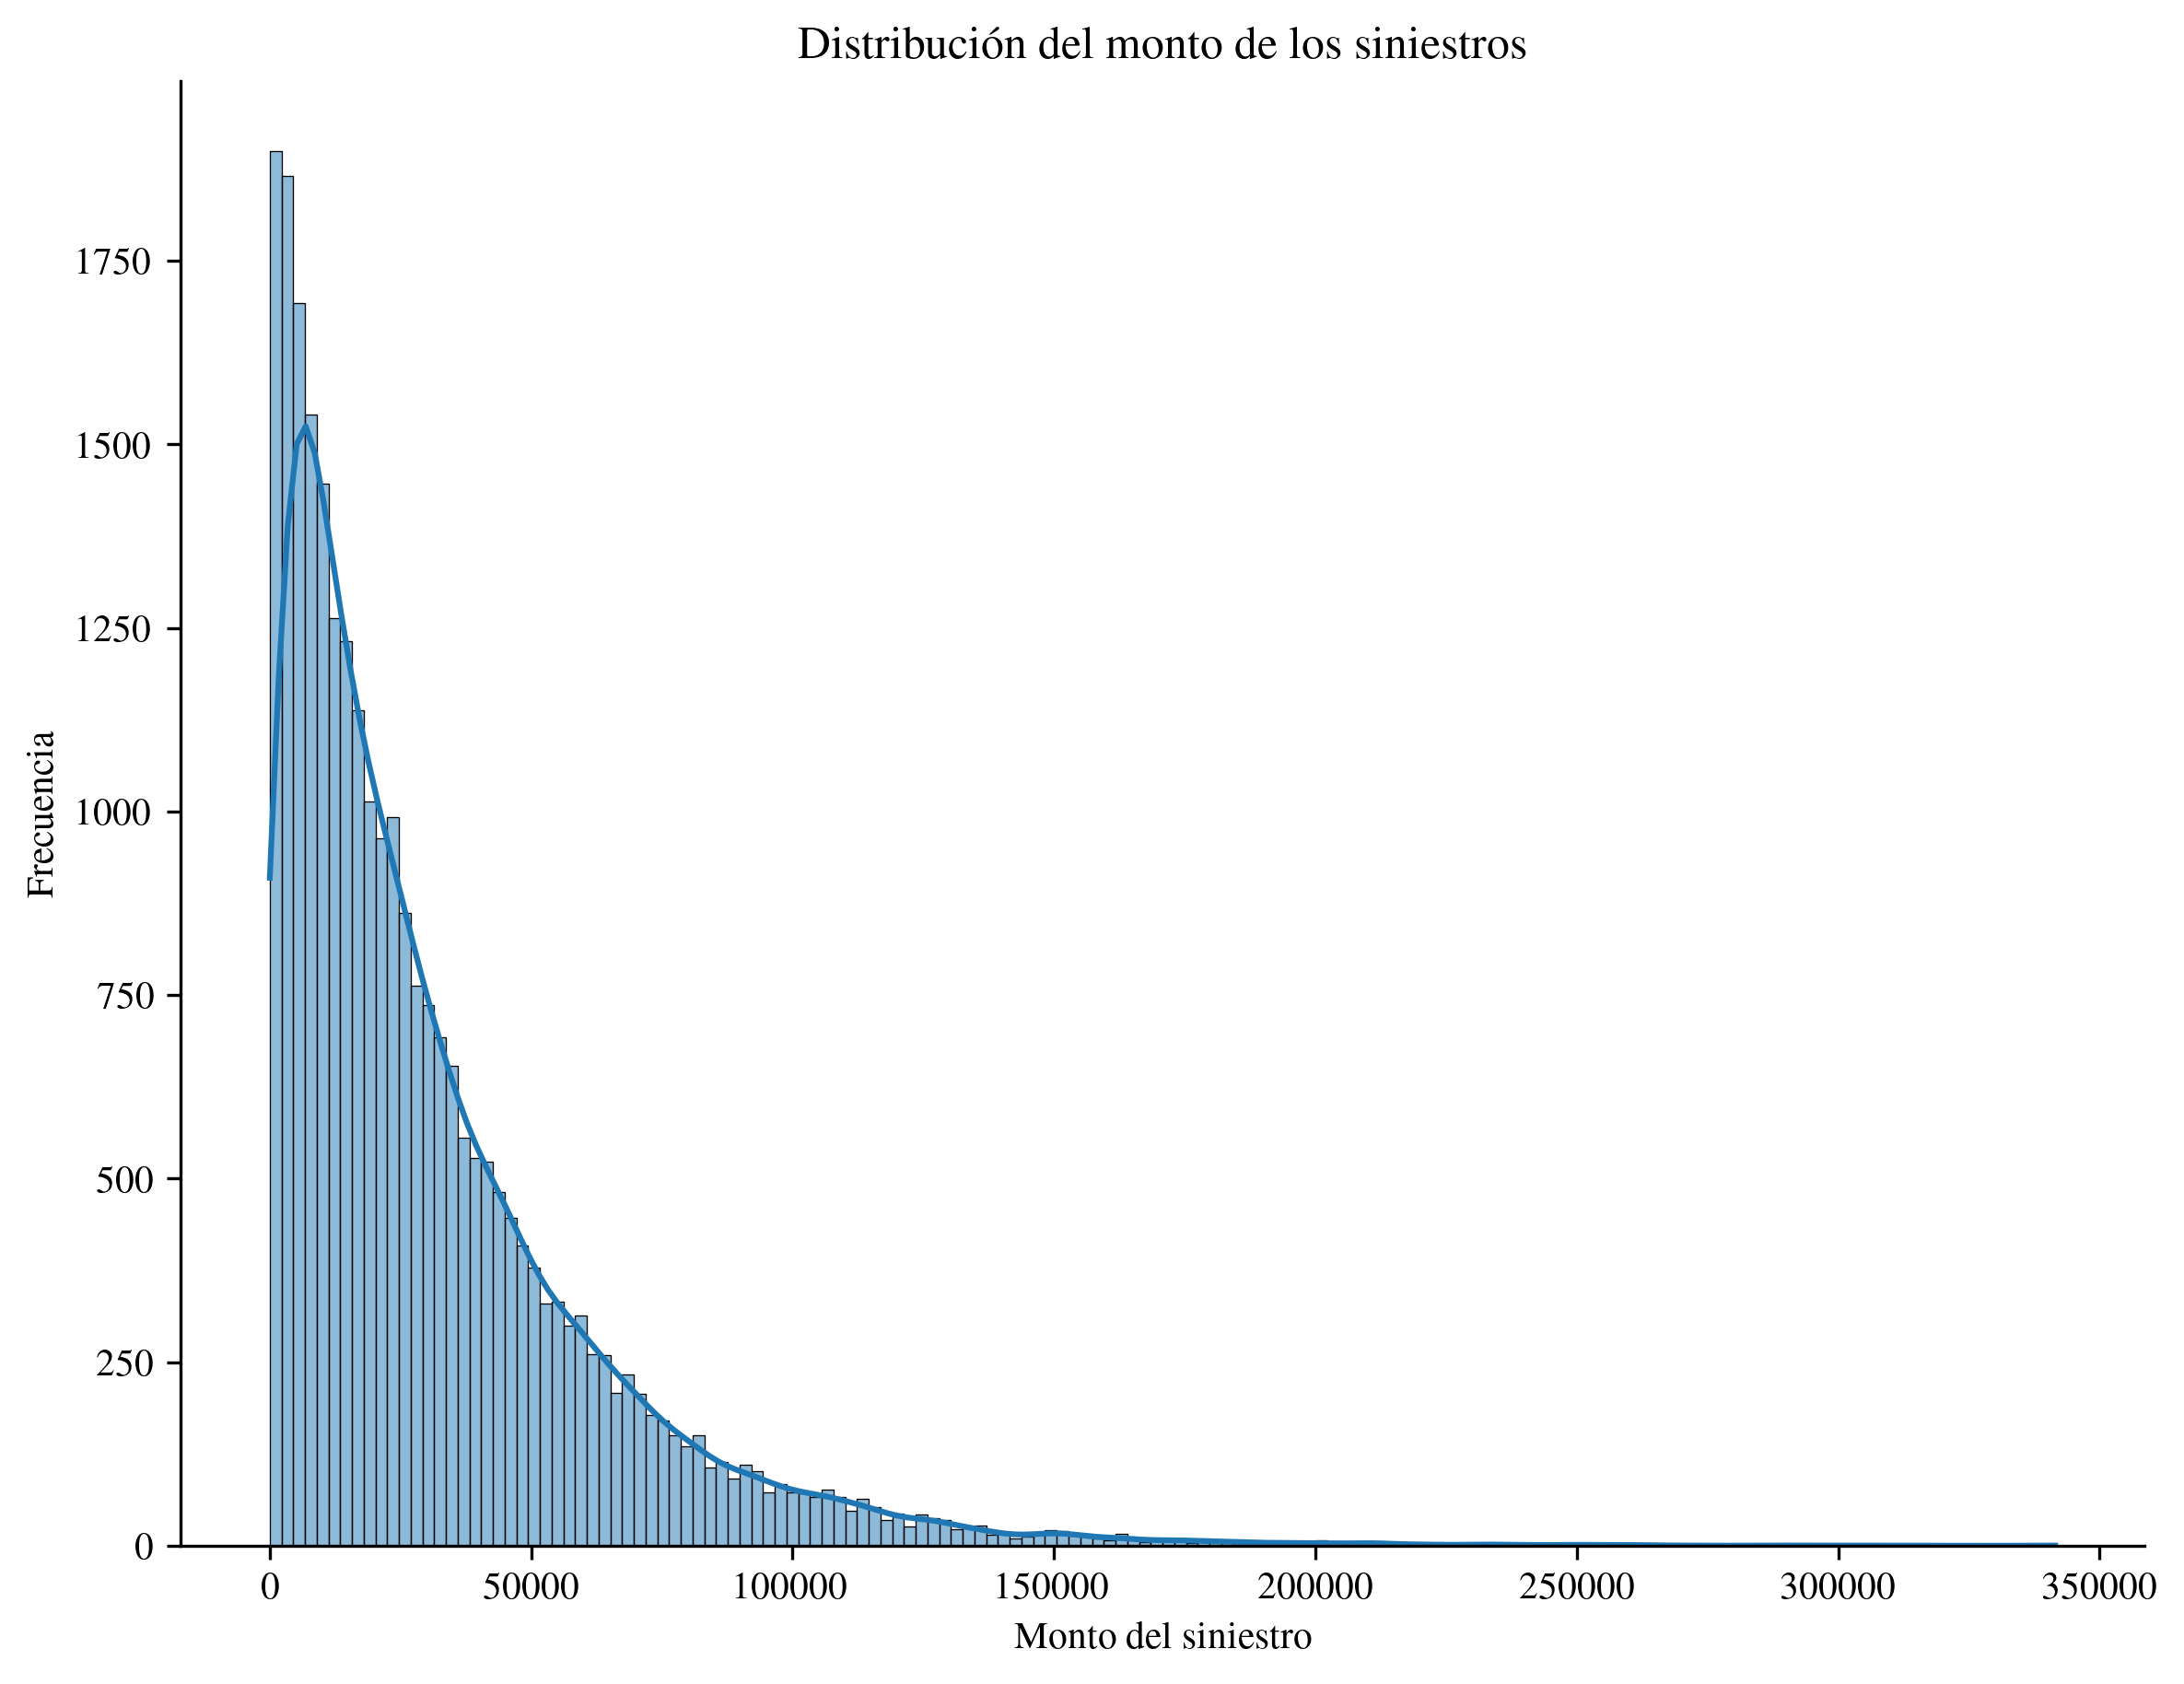
\includegraphics[scale=0.45]{img/amount_dist.png}
                    \caption{Distribución del monto de los reclamos}
                    \label{img:amount-dist}
                \end{figure}

                Para este estudio supondremos que esta variable aleatoria $Z$ sigue una distribución exponencial con un parámetro $\mu$.Para esta variable se hará la prueba de ajuste para la distribución exponencial con el mismo nivel de significancia $\alpha = 0.05$. Las hipótesis son las siguientes:
                \begin{gather*}
                    H_0: Z \sim\text{Exp}(\mu) \\
                    H_1 : Z \not \sim \text{Exp}(\mu)
                \end{gather*}
                
                El \textit{p-value} obtenido para la prueba de \emph{Lilliefors} fue de $0.09746$, y para la \textit{Anderson-Darling} fue $0.109$; ambas pruebas indican que no se puede rechazar la hipótesis nula, el modelado de esta variable aleatoria para nuestro caso de estudio será el de una distribución exponencial.
            
            \subsubsection{Discriminación de parámetros} \label{sec:parameter-estimation}
                    
                Ya que conocemos las distribuciones que modelan los fenómenos de interés, nos queda solamente estimar los parámetros de dichas distribuciones; como ambos son en este caso las medias poblacionales de cada variable, realizaremos 2 pruebas de hipótesis sobre la media poblacional, con un nivel de significancia $\alpha = 0.05$ para ambos casos.
                \begin{gather*}
                    H_0: \mu = \bar{\mu} \\
                    H_1: \mu \neq \bar{\mu}
                \end{gather*}
                \begin{gather*}
                    H_0: \lambda = \bar{\lambda} \\
                    H_1: \lambda \neq \bar{\lambda}
                \end{gather*}

                Para la prueba de la media del monto de los reclamos estimamos que la media poblacional $\mu$ es \$$30771.37$ con \texttt{p-value} de 1, para la media poblacional de reclamos por día $\lambda$ estimamos un valor de $74.30$ con un \texttt{p-value} de 1. Como estos valores no son menores que el nivel de significancia establecido, fallamos el rechazo de la hipótesis nula, y de ahora en adelante supondremos que estos son los parámetros de la distribuciones encontradas.
                
                El intervalo de confianza al $95\%$ de estos dos parámetros se puede calcular mediante la distribución normal (debido a que no se conoce la varianza poblacional de estos 2 parámetros). Los intervalos que hemos obtenido son:
                \begin{gather*}
                    \text{CI}_{\lambda} = \left(73.439, 75.169\right)\\
                    \text{CI}_{\mu} = \left(30,399.680, 31,143.071\right)
                \end{gather*}

                Por lo que cualquier $\lambda$ y $\mu$ dentro de estos intervalos darán un nivel de significancia del 5\% al modelo utilizar.

            \subsubsection{Cálculo de prima}

                Introducimos ahora una expresión para el cálculo de la prima que debe recibir la empresa aseguradora como una función del factor de recargo $\theta$; heurísticamente podríamos ver el factor de recargo como una medida de que tan elevada será la prima que la aseguradora le cobre a sus clientes. Se sabe que para que la probabilidad de ruina de la aseguradora no converja a 1, se tiene que cumplir la siguiente condición \cite{rolski2009stochastic}:
                \begin{equation}\label{eqn:no-ruin}
                    c > \lambda \mu
                \end{equation}

                De esta expresión podemos definir ahora la prima como una expresión en función de un parámetro $\theta$ que denominaremos \emph{factor de recargo}:
                \begin{equation}\label{eqn:def-theta}
                    c = (1 + \theta) \lambda \mu
                \end{equation}
                
                Para que se cumpla la restricción de la expresión \ref{eqn:no-ruin} $\theta$ tiene que ser estrictamente positivo. Para efectos de experimentación uno podría hacer este valor negativo pero no menor a $-1$ y observar como se comporta la probabilidad de ruina en las aproximaciones frecuentistas.

                El parámetro que proponemos es similar a la \emph{carga de seguridad} que la Dra. Ekaterina define en su artículo \cite{ekaterina}.

        \subsection{Simulación de probabilidad de ruina por Monte Carlo Crudo}

            Con los parámetros estimados en las secciones anteriores se realizará una simulación de la probabilidad de ruina mediante Monte Carlo Crudo. Nos interesará aproximar dicha probabilidad para un horizonte finito de tiempo $T$ mediante un número de simulaciones $N$. Nuestra estimación de la probabilidad de ruina para un capital inicial $U_0$ y un factor de recargo $\theta$ será la proporción de trayectorias en las que alguna vez el capital de la empresa $U_t$ fue menor a 0.

            Para dicha aproximación se calculará a su vez un intervalo de confianza al $95\%$ para después calcular su margen de error $ME$. El Socio Formador nos ha solicitado que dicho margen de error sea estrictamente menor a $0.05$. En caso de que el margen de error calculado sea mayor al estipulado, se incrementará el número de simulaciones $N$ hasta que satisfagamos las necesidades de la empresa aseguradora.

        \subsection{Cálculo de la probabilidad de ruina con fórmula de Pollaczek-Khinchine} \label{sec:pollaczek}

            Finalizaremos nuestro caso de estudio al obtener una expresión analítica para la probabilidad de ruina a un horizonte de tiempo infinito empleando la fórmula de \emph{Pollaczcek-Kinchine} \cite{josafat-santana-2020}; para su desarrollo supondremos que la frecuencia de los reclamos sigue un proceso de Poisson homogéneo de intensidad $\lambda$, y que la distribución que sigue el monto de los reclamos es una exponencial con parámetro $\mu$.

            La fórmula de \emph{Pollaczek-Khinchine} es un resultado obtenido al analizar el monto de superávit que generaría la empresa aseguradora \cite{burnecki2005best}, es decir:
            \begin{eqnarray*}
                Y(t) &=& u - U(t) = u-(u+ct-\sum_{k=1}^{N(t)} {Z_k}) \\
                &=& \sum_{k=1}^{N(t)} {Z_k} - ct
            \end{eqnarray*}

            Cuando $Z(t) > u$ se dice que la compañía ya quebró de igual manera cuando $U(t)<0$. Esto es debido a que 
            \begin{eqnarray*}
                U(t) &<& 0\\
                u + ct - \sum_{k=1}^{N(t)} {Z_k} &<& 0\\
                ct -\sum_{k=1}^{N(t)} {Z_k} &<& - u\\
                \sum_{k=1}^{N(t)} {Z_k} - ct &>& u\\
                Z(t) &>& u
            \end{eqnarray*}

            Ahora definamos $Y_k$ como sigue:
            \begin{equation}
                Y_k = \begin{cases}
                    \max{\{Z(t): Z(t)\geq0\}} \text{ si } k=0\\
                    \max{\{Z(t) : Z(t)\geq0\}} - Y_{k-1} \text{ si } k>0
                \end{cases}
            \end{equation}

            Por lo que la condición de ruina se puede escribir como sigue:
            \begin{equation}
                M = \sum_{k=0}^K Y_k \geq u
            \end{equation}

            La cual conlleva a la fórmula de \emph{Pollaczek-Khinchine}:
            \begin{equation}
                \psi (u) = P(M>u) = \frac{\theta}{1+\theta} \sum_{n=0}^\infty \left (\frac{1}{1+\theta}\right)^n \bar{B}_0^{*n}(u)
            \end{equation}

            En donde $\psi (u)$ es la probabilidad de ruina con horizonte infinito con utilidad inicial $u$. $\theta$ cumple que $c=(1+\theta)\lambda \mu$. $\bar{B}_0^{*n}(u)$ es la $n$-ésima convolución de la distribución cola de los reclamos \cite{taboga-2021}. La 0-ésima de $\bar{B}_0 (u)$ convolución se define en este caso es 0 si $u \geq 0$, y 1 si $u < 0$. La convolución, en el caso que $n=1$, se define como sigue:
            \begin{equation}
                \bar{B}_0^{*(1)}(u)=\bar{B}_0 (u)
            \end{equation}

            Y en caso de que $n > 1$:
            \begin{eqnarray*}
                \bar{B}_0^{*(n)}(u)&=&(\bar{B}_0^{*(n-1)} (u) * \bar{B}_0 (u))\\
                &=& \int _{-\infty}^{\infty} \bar{B}_0^{*(n-1)} (x) \bar{B}_0 (u-x) dx
            \end{eqnarray*}
    
            Si se sustituye $\bar{B}_0$ como la respectiva distribución cola de una exponencial se lleva a la siguiente fórmula para la probabilidad de ruina en un horizonte infinito \cite{josafat-santana-2020}:
            \begin{equation}\label{eqn:pollaczeck-prob}
                \psi(u) = \frac{1}{1+\theta} \cdot \exp\left(-\frac{u \theta}{(1+\theta)\mu}\right)
            \end{equation}

    \section{Experimentación y resultados} \label{sec:results}

        \subsection{Simulación de probabilidad de ruina por Monte Carlo Crudo} \label{sec:monte-carlo}

            Respondiendo a la primera de nuestras preguntas de investigación, se realizará una simulación de la probabilidad de ruina mediante Monte Carlo Crudo. Nos enfocaremos en estimar la probabilidad de ruina para un horizonte de tiempo $T$ de 5,000 días, y se realizarán 10,000 simulaciones $(N)$. Para esta simulación se usaron los parámetros $\lambda$ y $\mu$ estimados en la sección \ref{sec:parameter-estimation}, se supuso que la empresa aseguradora comenzó sus operaciones con un capital inicial $U_0 = 1,000,000$, y asignamos un factor de recargo $\theta = 0.05$, que resultó en una prima $c = 2,400,761.65$. Presentamos una visualización de las trayectorias simuladas en la figura \ref{fig:case-study-paths}.
            \begin{figure}[!htbp]
                \centering
                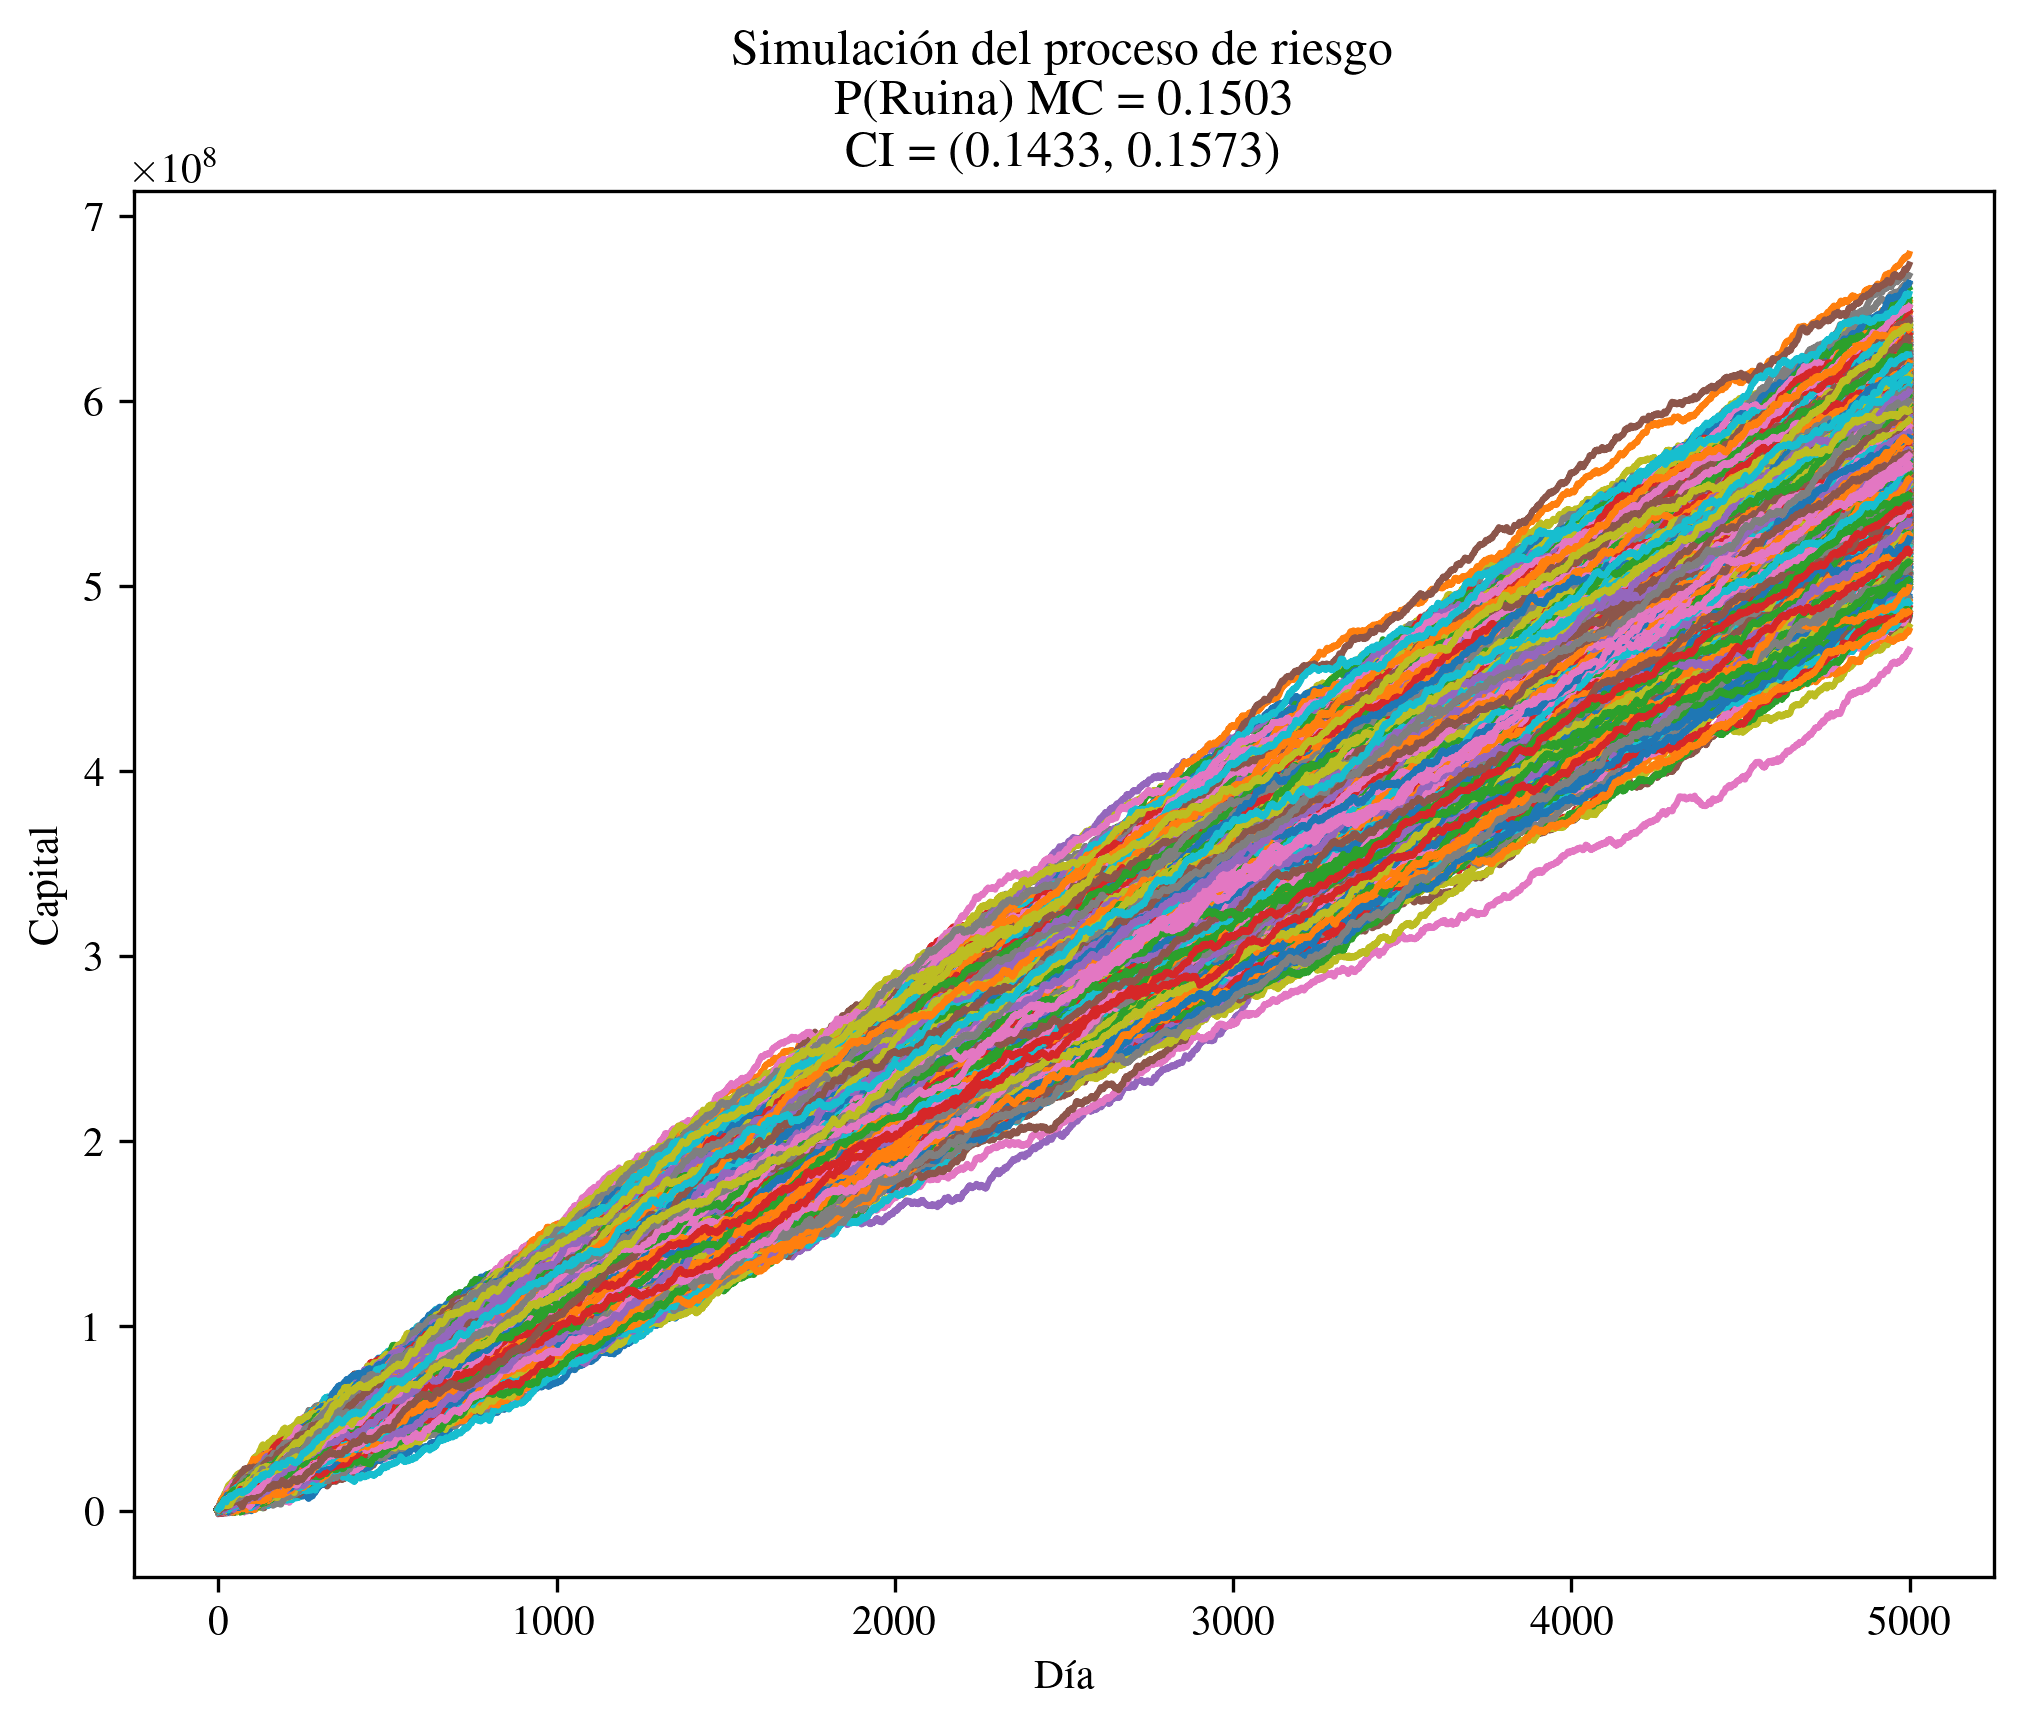
\includegraphics[scale=0.45]{img/ruin_sim_U01000000_T5000_Theta0.05_N10000.png}
                \caption{Trayectorias generadas de una simulación Monte Carlo Crudo, $\theta = 0.05$}
                \label{fig:case-study-paths}
            \end{figure}
            
            Para esta simulación hemos estimado una probabilidad de ruina $\bar{\psi}_{5000}(U_0) = 0.1503$. Hemos calculado también un intervalo de confianza al $95\%$ para esta proporción aprovechando el Teorema Central del Límite, obtuvimos un intervalo de confianza ${CI}_{\bar{\psi}} = \left(0.1433, 0.1573\right)$; el margen de error del intervalo de confianza fue $ME = 0.007$, que es menor al margen de error solicitado por el Socio Formador.

        \subsection{Cálculo de la probabilidad de ruina con la fórmula de Pollaczek-Khinchine} \label{sec:analytic-sol}

            Para resolver nuestra segunda interrogante, calcularemos la probabilidad de ruina para la empresa aseguradora para un tiempo infinito utilizaremos la ecuación \ref{eqn:pollaczeck-prob} que definimos en la sección \ref{sec:pollaczek}. Utilizaremos como capital inicial $u$ \$$1,000,000$, el factor de recargo $\theta$ se mantendrá en $0.05$ y el parámetro de la distribución exponencial del monto de los reclamos $\mu$ será el estimado en la sección \ref{sec:parameter-estimation}.
            
            Sustituyendo estos datos en la ecuación \ref{eqn:pollaczeck-prob} encontramos que la probabilidad de ruina a un horizonte infinito es $\psi(u) = 0.202$. Notamos que este valor difiere del que estimamos en la sección \ref{sec:monte-carlo}.

    \section{Discusión de resultados} \label{sec:discussion}

        A pesar de que el presente escrito ha cumplido con todas las especificaciones solicitadas por el Socio Formador, hemos encontrado algunas áreas de oportunidad que de ser resueltas añadirían aún más valor a nuestra investigación.

        \subsection{Complejidad computacional}

            El método de Monte Carlo Crudo que hemos usado en este trabajo se vuelve computacionalmente ineficiente cuando se quieren estimar probabilidades a horizontes de tiempo cada vez más grandes, su complejidad computacional de tiempo en el peor de los casos posibles es de orden $O(NT)$, para las especificaciones de nuestra investigación, nuestro algoritmo requeriría como máximo un total de $50,000,000$ de operaciones, tarea que se vuelve en extremo lenta cuando se usan lenguajes de programación dinámicos como lo es Python.

            Creemos que el uso de un lenguaje de programación más eficiente en conjunto con la implementación de un método de reducción de varianza, ayudarían a reducir la complejidad computacional de nuestras simulaciones a la vez que nos facilitan la estimación de probabilidades a horizontes de tiempo cada vez más grandes.

        \subsection{Diferencia entre probabilidad frecuentista y analítica}
            
            Como hemos observado en la sección \ref{sec:analytic-sol}, la probabilidad de ruina frecuentista que hemos obtenido mediante el proceso de simulación difiere de la calculada con la fórmula de \emph{Pollaczek-Khinchine} que hemos derivado para nuestro caso de estudio. Conjeturamos que este fenómeno ocurre ya que un horizonte de tiempo $T$ de 5,000 días no es lo suficientemente grande como para acercarse a la probabilidad analítica de que haya ruina en un horizonte infinito; sin embargo, para resolver este problema, se requeriría aumentar el horizonte $T$ y el número de simulaciones $N$ para garantizar un margen de error pequeño en nuestra estimación, lo que nos lleva de nuevo al área de oportunidad anterior.

    \section{Recursos utilizados} \label{sec:resources}

        La implementación del código fuente fue corrida en una máquina de sistema operativo Ubuntu 22.04.1 LTS x86\_64. El equipo disponía de un procesador Intel(R) Core(TM) i5-1035G1 CPU @ 3.6GHz, y tenía disponible 8 GB de RAM. Especificaciones sobre las versiones de los paquetes usados en este proyecto pueden ser encontrados en la documentación de nuestro repositorio \ref{sec:source-code}.
        
    \section{Conclusiones} \label{sec:conclusions}
        
        El análisis de la probabilidad de ruina seguirá siendo una de las principales tareas de la Teoría de Riesgo, el buen análisis de los registros históricos de una empresa en conjunción con la implementación de algoritmos de simulación eficientes es imperativo para cualquier departamento de gestión de riesgos.

        Dada la dificultad de encontrar fórmulas matemáticas cerradas para la probabilidad de ruina a horizontes de tiempo finitos, el uso de simulaciones como la que proponemos representa una buena alternativa para aquellas empresas que deseen entrar a este riesgoso mercado.

        La metodología desarollada solamente se vería beneficiada de la implementación de un mejor método de simulación que no tenga una complejidad computacional tan alta; esto le daría el poder a las aseguradoras de estimar la probabilidad de ruina de su empresa a largo plazo con un alto grado de fiabilidad.
    
    \appendices

    \section{Código Fuente} \label{sec:source-code}

        El código implementado puede ser consultado en el siguiente repositorio \href{https://github.com/JuanEcheagaray75/ruin-model}{aquí}.

    \nocite{*}
    \bibliographystyle{IEEEtran}
    \bibliography{references.bib}
    
\end{document}